\begin{v2}
\subsection{\label{sec:calib.cc}Cerenkov Calibration and Performance}

The Cerenkov detector's primary role in CLAS is to help differentiate leptons from pions at momentums below the pion Cerenkov radiation threshold.  The Cerenkov for g12 was roughly calibrated by importing the (then) most recent CLAS CC calibration constants and then verifying that the photoelectron number was reasonable on a sector by sector basis.  The following validation plots come from two g12 production runs skimmed only for pions via the standard PID, and inside the fiducial region as described in this document.  In Fig.~\ref{calib.cc_pesec} the total photoelectron yield for each sector is shown.  The histogram y-axis range is constant between all plots for ease of comparison.  One can see that the photoelectron yield is consistent between sectors.

\begin{figure}[htpb]
\begin{center}
 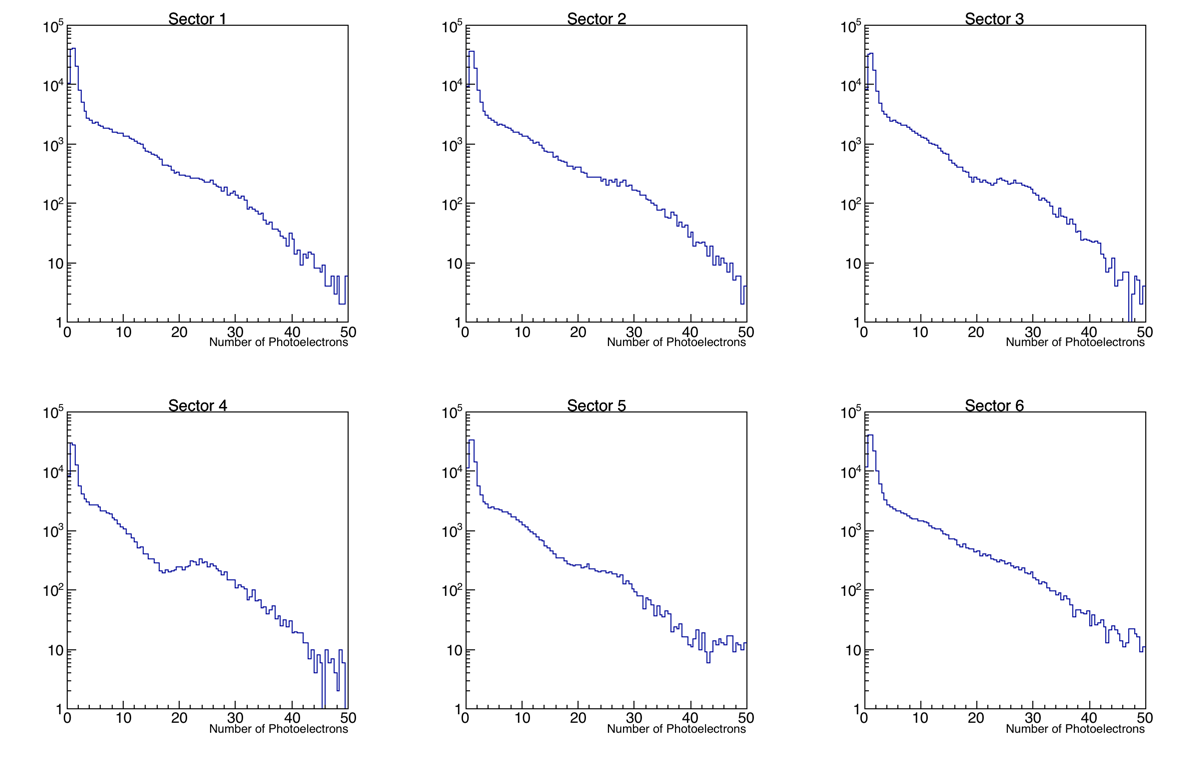
\includegraphics[width=0.75\textwidth]{figures/calib/cc/npeCC_check.png}
  \caption{An example CC photoelectron spectra from two production runs skimmed for pions.  The y-axis range is fixed over all plots for ease of comparison.}
  \label{calib.cc_pesec}
  \end{center}
\end{figure}

In Fig.~\ref{calib.cc_pepmt} the photoelectron yields are further broken down by PMT.  The z-axis (log-scale) is fixed for ease of comparison.  The important feature here is that the delta-ray "pion" peak in the photoelectron spectra peaks roughly around 1.0 photoelectrons for all PMTs. The general lepton selection criteria includes a cut > 2.5 photoelectrons, which is a relatively safe and conservative cut on any PMT (see Sec.~\ref{sec:data.lepton} for more details on the lepton PID).

\begin{figure}[htpb]
\begin{center}
 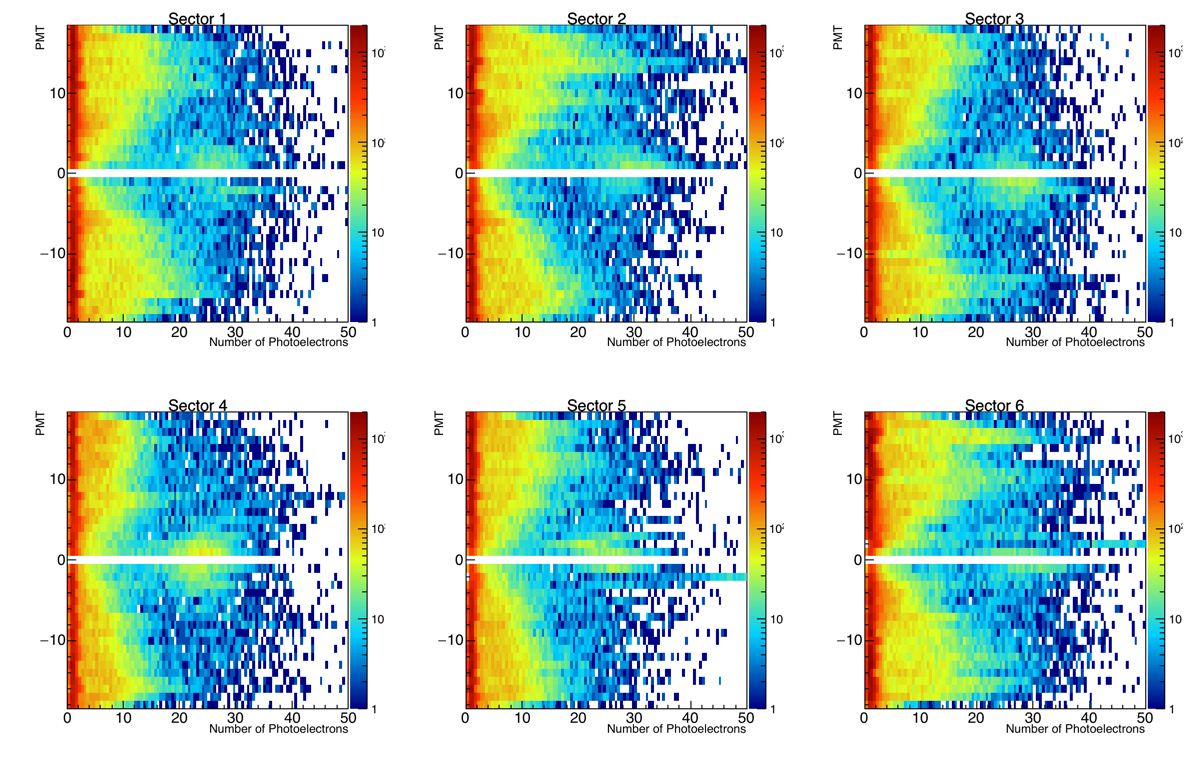
\includegraphics[width=0.75\textwidth]{figures/calib/cc/PMT_v_npe_log.png}
  \caption{Same plot as Fig.~\ref{calib.cc_pesec} but 2D in PMT number.  Negative and positive PMT numbers correspond to left and right CC PMTs. Z-axis range is fixed for ease of comparison.}
  \label{calib.cc_pepmt}
  \end{center}
\end{figure}

As an additional validity plot, the probability of a pion to cause a hit in the CC versus the momentum of the pion is shown in Fig.~\ref{calib.cc_piprob}.  This plot shows the expected behavior of the CC as the pions passes the Cerenkov radiation threshold.

\begin{figure}[htpb]
\begin{center}
 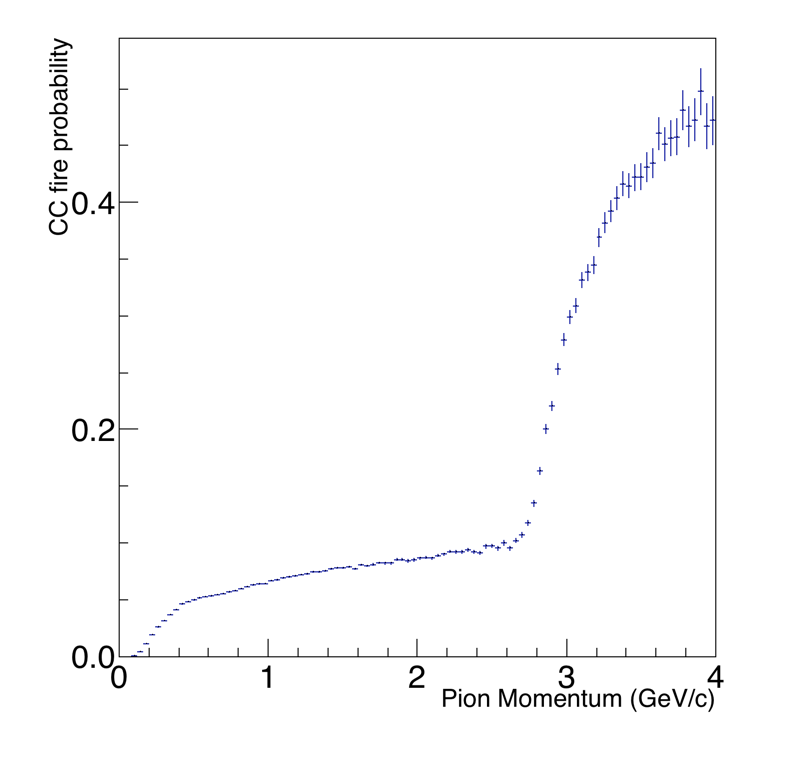
\includegraphics[width=0.45\textwidth]{figures/calib/cc/pionProb.png}
  \caption{The overall CC hit probability for pions within the fiducial region versus the pion momentum.}
  \label{calib.cc_piprob}
  \end{center}
\end{figure}


\subsubsection{\label{sec:calib.cc.eff}Cerenkov Efficiency}
The exact efficiency of the CC over all momenta and angles for leptons was never explicitly calculated.  Instead, it is recommended to look at the efficiency of the overall lepton identification procedure, if needed, for any lepton analyses.
\end{v2}

\FloatBarrier
